
\chapter{Testing the impacts of cells, nutrients, and organic matter released into the water column during sea ice melt}\label{ch:seaice}


\chapterdisclaimer{This work was performed in collaboration with Hugh Ducklow, Linda Amaral-Zettler, and Jeremy Rich.\\
\\
Catherine Luria, Linda Amaral-Zettler, Hugh Ducklow, and Jeremy Rich designed and conducted the study. Catherine Luria analyzed data and wrote this chapter with guidance from Jeremy Rich. 
}


\section{Abstract}

Sea ice is a key driver of seasonal and interannual ecosystem variability in the coastal waters of the Antarctic Peninsula. When sea ice, which harbors a rich microbial community, melts in the spring, microbes, organic material, and nutrients are released into the water column. We conducted a series of four mesocosm experiments during two austral springs to test the impacts of these inputs on water column bacteria. We found little support for the ``seeding hypothesis,'' the conjecture that algae released during ice melt form the basis of the intense algae blooms often seen in the marginal ice zone (MIZ). However, we did observe increased bacterial abundance and production in response to both whole and filtered sea ice additions, suggesting that bacteria responded favorably to a dissolved component of sea ice meltwater. The variation in results across our experiments was notable and reflects the heterogeneous nature of our sea ice inocula. 

\section{Introduction}

Sea ice is an integral part of polar ecosystems \citep{thomas2003sea, wywabdlc13}. It covers 7\% of the Earth's surface on a seasonal basis and plays a vital role in physical regulation of the marine environment and hence the marine food web \citep{Maycut1985-ng}. The pelagic ecosystem west of the Antarctic Peninsula (WAP) has experienced a 40\% decline in sea ice extent over the past few decades, with an overall trend toward later advance and earlier retreat, shortening the annual duration of sea ice cover by over 80 days \citep{Stammerjohn2008-nj}. Because the annual retreat and advance of sea ice profoundly influence numerous WAP ecosystem processes, as well as many species, minor shifts in temperature, which cause declines in sea ice duration and extent, can dramatically impact ecosystem function \citep{Clarke2008-zv}. In addition, decreased sea ice extent and duration reduces surface albedo and ice thickness, allowing for greater ocean winter heat flux, positively feeding back into trends toward warmer air temperatures and sea ice decline \citep{Ducklow2007-ns}.

Sea ice advance begins in the austral autumn with the formation of frazil ice crystals which incorporate carbon- and microbe-rich summer surface waters \citep{Garrison1996-ro}. As sea ice continues to coalesce, numerous microhabitats form including brine channels that perforate the bottom surface of the ice. These brine channels provide a stable growth platform for winter phytoplankton, allowing phytoplankton to remain near the surface and maximize exposure to limited light. The sea ice microbial community accounts for 9-25\% of primary production in the ice-covered Southern Ocean \citep{Arrigo1997-bj}. Ice algae form the base of a winter food web, creating a nutrient and carbon enriched niche that supports ice-inhabiting bacteria and zooplankton \citep{Garrison1989-sn}. The algae also support a winter population of juvenile krill that live directly under the ice and in turn support a variety of marine birds and mammals \citep{Ducklow2007-ns}. As such, declines in sea ice have the potential to impact all levels of the marine food web. Previous studies have examined the effects of sea ice extent and duration on primary production \citep{Vernet2008-on}, krill \citep{Ross2000-mm}, and seabirds \citep{Croxall2002-ja}. Summer phytoplankton biomass, and hence bacterial production are lower in years with less winter sea ice \citep{saba2014winter, dsvse12}. However, we know little about the direct impacts of annual sea ice retreat on bacteria in the WAP water column.

 

When sea ice retreats in the austral spring, in addition to releasing freshwater that contributes to water column stratification, it releases phytoplankton, bacteria, organic matter and nutrients. The ``seeding hypothesis'' proposes that the release of phytoplankton seeds the water column, forming the basis of spring phytoplankton blooms. Although the seeding hypothesis has not been extensively tested, previous microcosm experiments suggest that seeding alters phytoplankton abundance and community composition \citep{Kuosa1992-vk,Giesenhagen1999-kq}. The effects of the release of dissolved organic matter (DOM) and seeding by either bacteria or phytoplankton on bacterial community composition remain uncharacterized. Because microbes form the basis of the marine food web and contribute disproportionately to ecosystem function, the impact of sea ice retreat on the microbial community could have far-reaching effects. Furthermore, without understanding these impacts, we cannot predict how rapid declines in sea ice extent and duration may alter the WAP ecosystem. We conducted a series of mesocosm experiments to test the impacts of both filtered and unfiltered sea ice additions on microbial community production, biomass, and abundance. We hypothesized that while the release of DOM would enhance bacterial production and abundance, sea ice algae and bacteria are uniquely adapted to the sea ice environment and would not flourish in the water column after sea ice retreat. 

\section{Methods}

Mesocosm experiments were conducted in October and November of 2012 and 2013 at Palmer Station, Antarctica. For sea ice ``treatments,'' brown sea ice (i.e. sea ice that visibly contained algae and/or organic matter) was collected in acid-washed buckets from the surface at either Station B or from the shoreline around Palmer Station. The sea ice was melted in \SI{0.2}{\micro\meter} filter-sterilized seawater (50\% w/v) in order to avoid cell lysis at \textasciitilde{}1$^{\circ}$C or at room temperature while ensuring that the water temperature never rose above 0$^{\circ}$C. After the ice was completely melted, half of the meltwater was passed through \SI{0.22}{\micro\meter} polyethersulfone (EMD Millipore, Billerica, MA) filters for the ``filtered ice'' treatment, while the remainder of the melted sea ice solution was left unfiltered for the ``whole ice'' treatment. The filtered seawater, filtered sea ice solution and unfiltered sea ice solution were sampled prior to initiating experiments for chlorophyll \emph{a} (chl \emph{a}) and phaeopigment, bacterial and phytoplankton abundance, and bacterial production as previously described \citep{Luria2014-dj}.

For each experiment, acid-washed 50 L polycarbonate carboys were filled directly from a seawater intake located at a depth of 6 m, 16 m from the shore. The intake was sampled prior to any filtering on station. The mesocosm experiments contained three groups: 1) control (no amendments), 2) 1\% v/v filtered sea ice solution addition (testing the effects of dissolved carbon and nutrient additions), and 3) 1\% v/v unfiltered sea ice solution (testing the effects of microbial seeding). For each group, triplicate 50-L carboys were incubated at ambient seawater temperatures for 10 days. A volume ratio of 1:100 represents the melting of a 10-cm-thick layer of sea ice in a 10-m deep mixed layer. We sampled the carboys on days 0, 2, 4, 6, 8 and 10 for phytoplankton abundance through flow cytometry (2012 only), chl \emph{a} (2013 only), and bacterial abundance and production (both 2012 and 2013). All sampling took place at incubation temperatures. Chl \emph{a} and bacterial production were measured as described in Chapter 3. Autofluorescent particles (i.e. phytoplankton) were counted live immediately after sampling on an Accuri C6 flow cytometer (BD Biosciences, San Jose, CA) equipped with a blue laser beam (50 mW, 488 nm). Particle size was determined by forward scatter versus side scatter comparison with fluorescent microspheres (Polysciences, Inc., Washington, PA) of varying size (\SIrange{0.5}{20}{\micro\meter}) as previously described \citep{garzio2013microzooplankton}. Bacteria were stained with SYBR\textsuperscript{\textregistered} Green I (Invitrogen, Carlsbad, CA) as described in Chapter 3 and were counted using an Accuri C6 flow cytometer (BD Biosciences, San Jose, CA) in 2012 and a Guava easyCyte flow cytometer (EMD Millipore, Billerica, MA) in 2013. 

\section{Results} 

In 2012, sea ice nanophytoplankton (\SIrange{2}{20}{\micro\meter}) were very abundant, ranging from $1.5 \text{ to } 7.0 \times 10^{6}$ cells ml$^{-1}$, about two orders of magnitude greater than abundance in the underlying water column (Figure \ref{fig:ch5:exp2012}). Likewise, in 2013, sea ice chl \emph{a} ranged from \SIrange{19}{29}{\micro\gram\per\liter}, as opposed to \SIrange{0.1}{0.2}{\micro\gram\per\liter} in the underlying water column. Bacterial abundance ranged from $1.1 \text{ to } 1.4 \times 10^{9}$ cells ml$^{-1}$ in 2012 and from $9.5 \times 10^{5}$ to $3.4 \times 10^{6}$ cells ml$^{-1}$ in 2013. In the water column, bacterial production averaged around \SI{6}{\pico\mole \per\liter \per\hour}. In sea ice, production was higher in November of both years, reaching almost \SI{700}{\pico\mole \per\liter \per\hour} in November 2013. Filtration reduced nanophytoplankton abundance by 100\% (2012), chl \emph{a} concentration by 99.9\% or more (2013), and bacterial abundance by 99\% or more. Bacterial production was reduced by more than 99\% during the 2012 experiments and by 92-94\% during the 2013 experiments.


\begin{figure}[htbp] 
\centering 
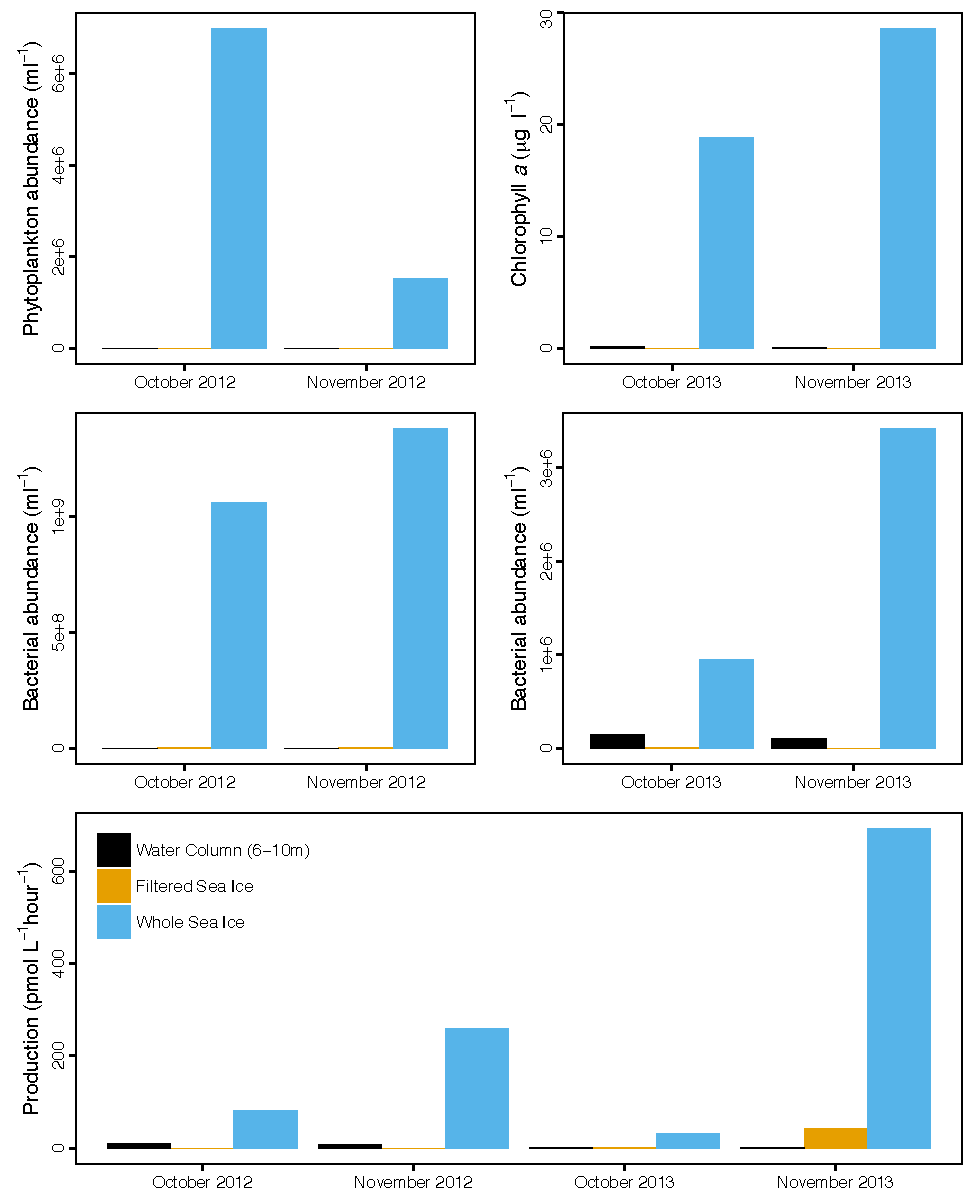
\includegraphics[width=0.9\textwidth]{Chapter_6_SeaIce/Figures/initial_values}
\caption{Initial phytoplankton abundance/biomass, bacterial abundance, and bacterial production values for filtered and unfiltered melted sea ice and the underlying water column.} 
\label{fig:ch5:exp2012} 
\end{figure}


During the October 2012 experiments, bacteria responded despite an apparent lack of phytoplankton growth under ice treatments (Figure \ref{fig:ch5:exp2013}). Nanophytoplankton abundance was actually greater in the control mesocosms for most of the experiment. Nonetheless, bacterial abundance and production increased substantially by Day 4 in both the filtered sea ice and whole sea ice mesocosms and remained higher through the rest of the incubation period. Likewise, in November 2012, nanophytoplankton abundance did not increase under sea ice treatments. Bacterial abundance was largely consistent across treatments. Bacterial production was greater on some days in the filtered ice mesocosms than in the control mesocosms. It was greater still in the whole sea ice mesocosms, and remained so throughout the experiment.

\begin{figure}[htbp] 
\centering 
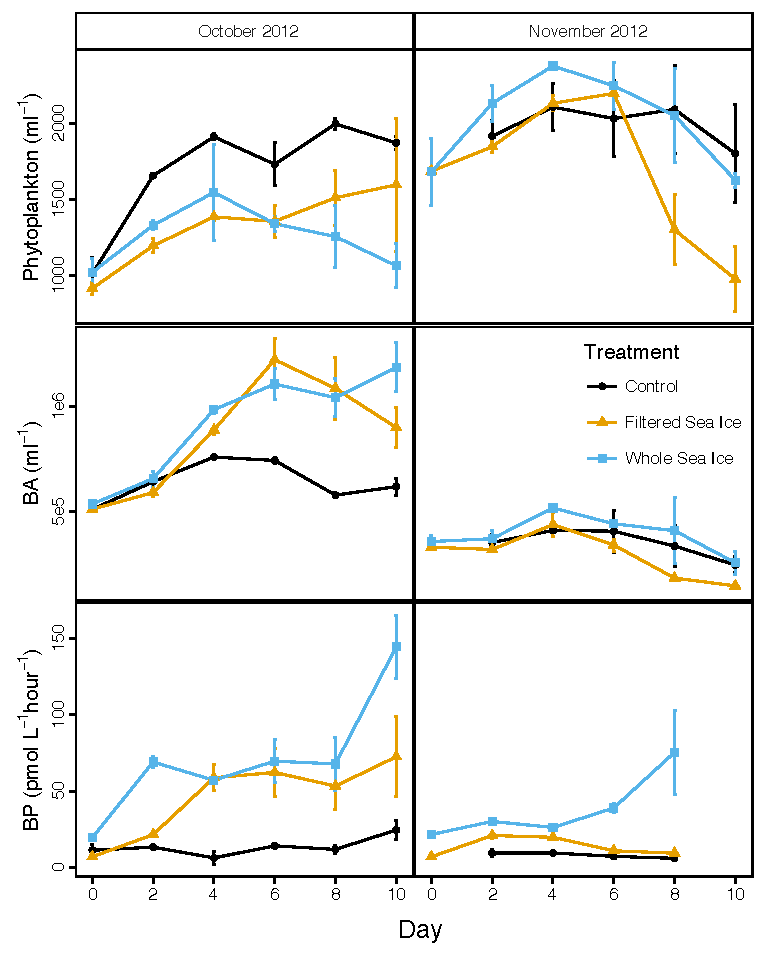
\includegraphics[width=0.9\textwidth]{Chapter_6_SeaIce/Figures/Experiments_2012}
\caption{Changes over a 10-day incubation period in phytoplankton abundance, bacterial abundance, and bacterial production in response to filtered and unfiltered sea ice additions, October and November 2012.} 
\label{fig:ch5:exp2013} 
\end{figure}

In contrast with the 2012 experiments, chl \emph{a} increased 2- to 7-fold under sea ice additions in both of the 2013 experiments (Figure \ref{fig:ch5:initial}). Chl \emph{a} was \textasciitilde{} \SI{0.2}{\micro\gram\per\liter} in the control and \textasciitilde{}\SI{0.8}{\micro\gram\per\liter} in the whole sea ice mesocosms at the initiation of the October experiment. It remained fairly stable in the control mesocosms, but reached \SI{1.3}{\micro\gram\per\liter} in the whole sea ice mesocosms by the end of the experiment. Chl \emph{a} started and ended lower in both the control and whole sea ice mesocosms in the November experiment compared to the October experiment, but levels in the whole sea ice mesocosms were still higher than in the control. Bacterial abundance was higher in both the filtered ice and whole ice mesocosms in October 2013. It was higher in the whole ice mesocosms only on days 2 and 4 in November 2013. Bacterial production was greatest in the filtered sea ice mesocosms on Day 2 in October 2013 and in the whole sea ice mesocosms in November 2013, but the trends were inconsistent and any changes were minor relative to those observed during the 2012 experiments.

\begin{figure}[htbp] 
\centering 
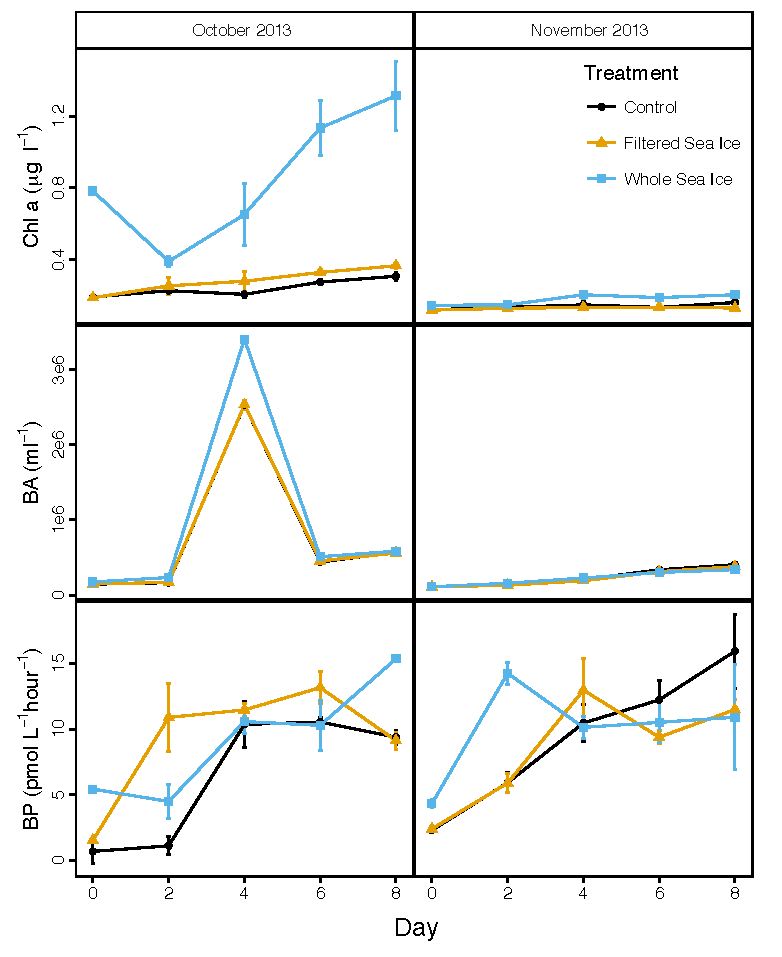
\includegraphics[width=0.9\textwidth]{Chapter_6_SeaIce/Figures/Experiments_2013}
\caption{Changes over a 8-day incubation period in phytoplankton biomass (chlorophyll \emph{a}), bacterial abundance, and bacterial production in response to filtered and unfiltered sea ice additions, October and November 2013.} 
\label{fig:ch5:initial} 
\end{figure}

\section{Discussion}

Phytoplankton blooms often track the receding ice edge in the spring \citep{Smith1985-lx,Smith1986-en} and summer phytoplankton biomass is greater in areas and in years with heavy winter sea ice \citep{Nicol2000-gd,saba2014winter}, giving rise to the ``seeding hypothesis'' in which inoculation of the water column by cells released from sea ice initiates phytoplankton blooms \citep{Garrison1989-sn,Garrison2007-ea}. Shared dominant species in sea ice and the neighboring MIZ provide support for this hypothesis \citep{Garrison1989-sn,Garrison1985-yg,Lannuzel2013-gk,Smith1986-en}. The increased chl \emph{a} in whole sea ice mesocosms in our 2013 experiments suggests that phytoplankton released from sea ice do in fact proliferate to an extent in the water column. However, the changes in phytoplankton biomass and abundance that we recorded were minor compared to changes during phytoplankton blooms in the environment. 

Sea ice contains abundant algal populations, with chl \emph{a} concentrations that can reach tens and hundreds of mg m$^{-3}$, and the presence of similar species in the MIZ suggests that sea ice is not necessarily populated by organisms that thrive exclusively in ice \citep{Garrison2007-ea}. However, numerous factors could influence the viability of potential seed populations within the ice. Meteorological and oceanographic conditions can affect the physical structure of sea ice \citep{Ackley1994-ld}, and subsequently algal access to nutrients and inorganic carbon \citep{Fritsen1994-zw,Gleitz1995-un}. Salinity varies greatly in sea ice; very high salinities can inhibit phytoplankton growth while very low salinity may lead to cell lysis \citep{Etheridge2005-vg,Garrison1985-yg}. The accumulation of low-salinity meltwater within or beneath the ice could lead to mass algal mortality during the melting process \citep{Lizotte2008-un}. In addition, a large fraction of ice algae have been shown to form aggregates, resulting in rapid sedimentation during melting \citep{Giesenhagen1999-kq,Riebesell1991-xy}. Perhaps, as a result, some studies have found that only small ice algae (<\SI{10}{\micro\meter}) persist in the water column \citep{Mathot1991-nv}. Together, these factors may alter the viability and species composition of the sea ice biota and the likelihood that this community will proliferate upon release into the water column. 

Whole sea ice additions actually reduced phytoplankton abundance in one of our experiments. \citet{Mathot1991-nv} and \citet{Lannuzel2013-gk} attribute reduced phytoplankton abundance during similar experiments to grazers. Heterotrophic species of chrysophytes, cryptophytes, and euglenophytes have been reported in sea ice \citep{Ikavalko1997-ak,Lizotte2008-un} and high grazing pressure was observed at the ice edge in the Weddell Sea \citep{Riebesell1991-xy}. Likewise, high virus counts were found in association with an ice algal bloom in the Arctic \citep{Maranger1994-uk}. Algal blooms within the ice itself, which can occur as light availability increases in the spring, increase the size of the potential seed community, but they may also increase the abundance of grazers just as sea ice is receding \citep{Leu2015-at}. 

Overall, our results suggest that the effects of seeding are quite minor. Previous studies based on mesocosm experiments provide conflicting evidence on this topic, reporting variously that that seeding effects are negligible \citep{Riebesell1991-xy}, patchy \citep{Kuosa1992-vk}, or substantial \citep{Giesenhagen1999-kq,Lannuzel2013-gk}. Therefore, we suspect that the physical changes wrought in the upper water column by sea ice retreat are of far greater significance to MIZ blooms. Sea ice melt freshens surface waters and subsequent shoaling of the upper mixed layer allows phytoplankton to persist and proliferate in the euphotic zone are far more significant than inconsistent seeding effects \citep{saba2014winter,Venables2013-me,Vernet2008-on}. The impact of water column stratification and potential interactions between stratification and seeding are impossible to test on the mesocosm scale.

While we found little evidence of phytoplankton seeding, we did observe bacterial responses to sea ice that were independent of sea ice-induced phytoplankton growth (c.f. \citealt{Lannuzel2013-gk} and \citealt{Giesenhagen1999-kq}). These responses were actually stronger in 2012 when we detected little, no, or even negative phytoplankton growth under sea ice treatments. Response levels were usually, but not always, similar between whole sea ice and filtered sea ice mesocosms, suggesting that bacteria reacted to an element found in the dissolved fraction of sea ice melt water (i.e. nutrients or organic matter). WAP bacterial growth is thought to be primarily limited by the availability of labile DOM \citep{dsvse12,Kirchman2009-sg}, which accounts for a large fraction of sea ice primary production \citep{Gosselin1997-qs}. Sea ice DOM might be especially abundant if mortality rates were high during melting. Ice DOM could be particularly important to bacteria as it enters the system in the spring before primary production in the water column partially relieves DOM limitation. While macronutrients are seldom limiting in the WAP region, micronutrients accumulated in sea ice may also stimulate growth \citep{Martin1990-ly}. For example, \citep{Loscher1997-ii} reported that iron concentrations were 2 to 100 times higher in sea ice than in the surrounding surface water. Therefore, sea ice melt water could have strong impacts on both bacterial and phytoplankton growth separate from the influences of seeding and water column stratification.

An insight from our results is the high degree of variability in our sea ice inocula and in subsequent impacts on bacterial growth. Phytoplankton biomass and bacterial production and abundance in the sea ice varied substantially between years and even between months within a single year. Bacteria responded more strongly to sea ice additions in 2012 than in 2013 and differences between the whole sea ice and filtered sea ice mesocosms were not consistent. A small body of papers report similar studies testing the the mechanisms controlling ice-edge plankton blooms, each tailored to address specific questions \citep{Giesenhagen1999-kq,Kuosa1992-vk,Lannuzel2013-gk,Riebesell1991-xy}. Significant variation in results between studies and between experiments within a single study is evident, and is sometimes attributed, as in our study, to differences in the original ice \citep{Kuosa1992-vk}. Experiments testing the effects of sea ice meltwater on marine microbes, as well as models of the large-scale impacts of sea ice melt on the marine environment must account for this high degree of heterogeneity in sea ice characteristics.

